\section{Lernfeld 6 - Programmieren}

%%% Anfang: tl;dr
\subsection{tl;dr - Zusammenfassung der Zusammenfassung}
%%% Ende: tl;dr
%%%%%%%%%%%%%%%%%%%%%%%%%%%%%%%%%%%%%%%%%%%%%%%%%%%%%%%%%%%%%%%%%%%%%%%%%%%%%%%%

%%% Anfang: HTML / PHP
\subsection{Einführung in HTML und PHP}

HTML ist, wie der Name -- HyperText Markup Language -- schon sagt, eine Beschreibungsssprache. Der aktuelle Standard lautet HTML 5 und basiert auf XHTML. Im Gegensatz zu Word sieht das interpretierte Ergebnis eines HTML-Dokuments nicht so aus, wie sie geschrieben wurde. HTML ist also eher mit \LaTeX zu vergleich. Das heißt, HTML ist keine Programmiersprache.

In den folgenden Abschnitten werden zunächst die wichtigsten Tags beschrieben, um HTML-Dokumente zu strukturieren. Anschließend werden die Möglichkeiten von HTML anhand von Aufgaben und deren Lösungen dargestellt.

%%% Anfang: LS01 > Kurzreferenz
\subsubsection{HTML5: Kurzreferenz}
In diesem Abschnitt werden die wichtigsten Tags beschrieben, um ein HTML-Dokument zu strukturieren. Alle erwähnten Dateien befinden sich unter \texttt{code/lf06prog-code}.\newline

{\bf Überschriften}.\ \ Ähnlich wie in TeX können Überschriften in mehreren Ebenen beschrieben werden. Wo TeX bloß drei Ebenen vorsieht (\verb+\section, \subsection} und \subsubsection+), sind durch HTML prinzipiell keine Grenzen gesetzt. Überschriften werden in HTML durch die Tags \texttt{<hX>} und \texttt{</hX>} beschrieben. Dabei steht X für die jeweilige Hierarchie. Abhängig von X wird die Größe der Überschrift gesetzt. Die Datei \texttt{lf06prog-headlines.html} macht das Beschriebene anschaulich.\newline

{\bf Absätze}.\ \ Möchte man einen Textblock als zusammengehörigen Absatz definieren, setzt man dafür die Tags \texttt{<p>} und \texttt{</p>}. Harte Zeilenumbrüche werden durch das einzelne Tag \texttt{<br />} beschrieben. Weil zwischen den Tags \texttt{<br> <br/>} eh nichts steht, wurde dieses vereinfacht. Daher ist auf das Leerzeichen in \texttt{<br />} zu achten.\newline

{\bf Hervorhebungen}.\\
\begin{tabular}{lll}
\texttt{<b> </b>} & {\bf fett} (physikalisch $\widehat{=}$ Stilelement) & \\
\texttt{<strong> </strong>} & {\bf fett} (logisch $\widehat{=}$ wichtig) & \\
\texttt{<i> </i>} & {\it kursiv} & \\
\texttt{<em> </em>} & betont; meist {\it kursiv} & \\
\texttt{<sup> </sup>} & $^{hochgestellt}$ & \\
\texttt{<sub> </sub>} & $_{tiefgestellt}$ & \\
\texttt{<u> </u>} & \sout{durchgestrichen} & \\
\end{tabular}\newline

{\bf Listen}.\ \ Mit den Tags \texttt{<ul> </ul>} und \texttt{<ol> </ol>} lassen sich Listen definieren. \texttt{<li> </li>} definieren jeweils die Listenelemente, wobei den Listenelementen bei \texttt{<ul>} ein Punkt vorangestellt wird und bei \texttt{<ol>} die Listenelemente durchnummeriert werden. Siehe dazu auch \texttt{lf06prog-listen.html} und \url{http://wiki.selfhtml.org/wiki/HTML/Textstrukturierung/Listen}.\newline

{\bf Umlaute}.\ \ HTML kann Umlaute nicht ohne weiteres darstellen. Daher müssen Umlaute durch die folgenden Befehle definiert werden:\\
\begin{tabular}{ll}
ä & \&auml;\\
Ä & \&Auml;\\
ö & \&ouml;\\
Ö & \&Ouml;\\
ü & \&uuml;\\
Ü & \&Uuml;\\
ß & \&szlig;\\
\euro & \&euro;\\
\end{tabular}\newline

{\bf Tabellen}.\ \ Besondere Bedeutung in HTML haben Tabellen. Mit diesen lässt sich der Aufbau einer Seite gestalten. Statt den Aufbau von Tabellen umständlich zu beschreiben, verweise ich auf die Datei \texttt{lf06prog-listen.html}. Diese sollte sich sowohl als Quellcode als auch im Browser angesehen werden.\newline

{\bf Links}. . .\ \ sind einer der großen Fortschritte, die das Internet erst zu dem machen, was es ist.
\begin{tabular}{lll}
Interner Link & \verb+<a href="interner-link.html">Beschreibung</a>+ &\\
Externer Link & \verb+<a href=\"https://externer-link.html\">Beschreibung</a>+ &\\
Link auf Bild & \verb+<a href=\"lokales-bild.jpg\">Bild</a>+ &\\
Link auf PDF & \verb+<a href=\"lokales-pdf.pdf\">Beschreibung</a>+ &\\
Mail als Link & \verb+<a href=\"mailto:email@email.email\">Schreib mich an!</a>+ &\\
Sprungmarke & \verb+<a href="\#anker">Spring zu Anker</a>+ &\\
& benötigt: \verb+<a name=\"anker\">Anker</a>+ &\\
\end{tabular}\newline

{\bf Grafiken}.\\
\verb+<img src="bild.jpg" width="" height="" border="0" alt="" title="" />+\\
\begin{tabular}{ll}
src & Wo die Datei liegt\\
width & Wie breit das Bild dargestellt werden soll\\
height & Wie hoch das Bild dargestellt werden soll\\
border & Rahmen?\\
alt & Beschreibung des Bildes\\
title & Titel des Bildes\\
\end{tabular}\newline

{\bf Kommentare}. . .\ \ lassen sich in HTML-Dokumenten einfügen, indem sie zwischen \verb+<!-- -->+ geschrieben werden.

%%% Ende: HTML-Kurzreferenz
%%%%%%%%%%%%%%%%%%%%%%%%%%%%%%%%%%%%%%%%%%%%%%%%%%%%%%%%%%%%%%%%%%%%%%%%%%%%%%%%

%%% Anfang: PHP
\subsection{PHP}

PHP ist eine Skriptsprache und basiert auf der C-Syntax.

Zur Erleichterung der Lesbarkeit von PHP-Code sollte die Formatierung der hier verwendete Beispiele verwendet werden.

%%% Anfang: PHP > Quotation
\subsubsection{Quotation unter PHP}

PHP unterscheidet wie die Bash zwischen schwacher und starker Quotation. Schwache Quotation bedeutet, dass Funktionen innerhalb der Anführungszeichen \" interpretiert werden. Das bedeutet, dass Variablennamen aufgelöst werden und statt ihrer der entsprechende Werte ausgegeben wird. Starke Quotation lässt sich mit einfachen Anführungszeichen \' umsetzen. Innerhalb der einfachen Anführungszeichen werden die Funktionen nicht interepretiert, sodass statt des Wertes der Variablenname ausgegeben wird. Im Listing [Nr] befindet sich ein Beispiel für schwache und starke Quotation in PHP.

\lstinputlisting
	[basicstyle=\small,showstringspaces=false,caption={Indexadressierte Arrays in PHP}
	\label{lst:array-index},captionpos=b,language=PHP]
	{code/lf06prog-code/lf06prog-array-index.php}
	
Möchte man sowohl den Variablennamen als auch den Wert ausgeben, lässt sich die Quotation auch unterbrechen. Dies ist im dritten \texttt{echo}-Befehl des Listings zu sehen. Die Punkte vor und nach dem Variablennamen bedeuten, dass der Inhalt der Variable der Ausgabe angehängt wird.

%%% Ende: PHP
%%%%%%%%%%%%%%%%%%%%%%%%%%%%%%%%%%%%%%%%%%%%%%%%%%%%%%%%%%%%%%%%%%%%%%%%%%%%%%%%

%%% Anfang: Formulardaten
\subsection{Formulardaten}

%%% Anfang: Formulardaten > HTML
\subsubsection{Formulardaten: HTML}

Im Listing [Nr] steht \texttt{action="\ script.php"}. Dies bezieht sich auf den Namen des Skriptes, an welches die Formulardaten beim Drücken auf den Submit-Button weitergereicht werden sollen.

\lstinputlisting
	[basicstyle=\small,showstringspaces=false,caption={Ein Beispiel für den HTML-Teil von Formulardaten}
	\label{lst:html-formulardaten},captionpos=b,language=HTML]
	{code/lf06prog-code/lf06prog-formulardaten.html}

Als \texttt{method} lässt sich \texttt{POST} oder \texttt{GET} wählen. Der Unterschied zwischen \texttt{POST} und \texttt{GET} besteht darin, dass die Formulardaten von \texttt{GET} in der URL auftauchen. Dadurch werden die geforderten Daten sichtbar und durch brute force angreifbar. Ein weiterer Nachteil von \texttt{GET} besteht darin, dass die übergebenen Daten nicht größer als 2KB sein dürfen. Diese Nachteile und Beschränkungen gelten nicht für \texttt{POST}. Daher ist \texttt{POST} zu bevorzugen.

Der wichtigste Teil, um Formulardaten abzufragen, sind die Felder, in denen sie eingetragen werden können. Die Felder lassen sich wie im Listing gezeigt mit \texttt{<input .../>} einfügen. Beispielsweise kann mit dem type \texttt{text} ein String in der Variable \texttt{txt\_variablenname} an das oben genannte Skript übergeben werden.
\begin{itemize}
	\item \texttt{text}: der type \texttt{text} nimmt noch weitere Attribute, wie bspw. \texttt{size} und \texttt{maxlength}. Ersteres gibt die sichtbare Länge des Feldes an und letzteres die maximale Länge des Inputs.
	\item \texttt{radio}: auch hier gilt, dass mit dem \texttt{name} der Variablenname definiert wird. Darüber hinaus beschreibt \texttt{value} den Wert, den die Variable annimmt, wenn der Radiobutton angeklickt wird.
	\item \texttt{submit}: im Gegensatz zum type \texttt{radio} beschreibt \texttt{value} hier die Beschriftung des Submit-Buttons.
\end{itemize} 

%%% Anfang: Formulardaten > PHP
\subsubsection{Formulardaten: PHP}

Das nächste Listing zeigt, wie die Formulardaten in PHP verarbeitet werden können. Zu Anfang des Listings findet sich der Bereich \ql Variablen setzen\qr. Diese Aufteilung ist nicht notwendig, sondern vereinfacht nur die Les- und Wartbarkeit des Codes. Sollten sich die Variablennamen später einmal ändern, muss nur die eine Zuweisung angepasst werden und nicht jedes Vorkommen der Variable.

\lstinputlisting
	[basicstyle=\small,showstringspaces=false,caption={Ein Beispiel für den PHP-Teil von Formulardaten}
	\label{lst:html-formulardaten},captionpos=b,language=PHP]
	{code/lf06prog-code/lf06prog-formulardaten.php}

%%% Anfang: Strukt. Programmierung
\subsection{Strukturierte Programmierung}
Strukturierte ist ein programmiersprachenübergreifendes Programmierparadigma. Es beinhaltet zum einen die baumartige Zerlegung eines Programms in Teilprogramme und enthält somit das Paradigma der prozeduralen Programmierung. Zum anderen verlangt die strukturierte Programmierung auf der untersten Ebene die Beschränkung auf drei Kontrollstrukturen: (1) Sequenzen, (2) Verzweigung und (3) Schleifen.

%%% Ende: Strukt. Programmierung
%%%%%%%%%%%%%%%%%%%%%%%%%%%%%%%%%%%%%%%%%%%%%%%%%%%%%%%%%%%%%%%%%%%%%%%%%%%%%%%%

%%% Anfang: Struktogramm
\subsection{Programmablaufplan und Struktogramm}

{\bf Programmablaufplan (PAP)}~\\

Ein Programmablaufplan (PAP) (auch Flussdiagramm, engl. {\it flowchart}) ist eine graphische Darstellung von Algorithmen in einem Programmen und beschreibt die Operationen zur Lösung einer Aufgabe. Die Symbole für Programmablaufpläne sind in der DIN 66001 genormt. Dort werden auch Symbole für Datenflusspläne definiert. Im Bereich der Softwareerstellung werden sie nur noch selten verwendet: Programmcode moderner Programmiersprachen bietet ähnlichen Abstraktionsgrad, ist jedoch einfacher zu erstellen und in der Regel sehr viel einfacher zu verändern als ein Ablaufdiagramm.

Das Konzept der Programmablaufpläne stammt, ebenso wie das etwas jüngere Nassi-Shneiderman-Diagramm (Struktogramm), aus der Zeit des imperativen
Programmierparadigmas.

{\bf Elemente:}\\
\begin{itemize}
	\item Oval: Start/Stopp\\
		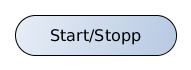
\includegraphics[scale=0.5]{pictures/lf06prog-pic/lf06prog-pap-start-stopp.png}
	\item Pfeil/Linie: Verbindung zum nächstfolgenden Element\\
		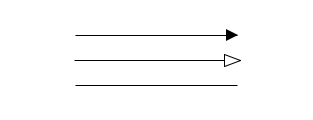
\includegraphics[scale=0.5]{pictures/lf06prog-pic/lf06prog-pap-pfeil.png}
	\item Rechteckt: Operationen\\
		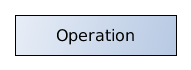
\includegraphics[scale=0.5]{pictures/lf06prog-pic/lf06prog-pap-operation.png}	
	\item Rechteck mit doppelten, vertikalen Linien: Unterprogrammaufruf\\
		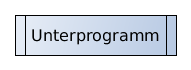
\includegraphics[scale=0.5]{pictures/lf06prog-pic/lf06prog-pap-unterprogramm.png}	
	\item Raute: Verzweigung\\
		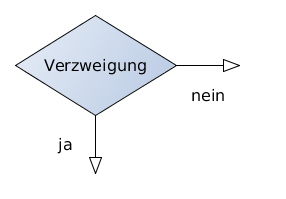
\includegraphics[scale=0.5]{pictures/lf06prog-pic/lf06prog-pap-verzweigung.png}	
	\item Parallelogramm: Ein- und Ausgabe (nicht nach DIN 66001 1983!)\\
		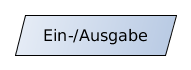
\includegraphics[scale=0.5]{pictures/lf06prog-pic/lf06prog-pap-ein-ausgabe.png}	
	\item Ergänzung: Schleife\\
		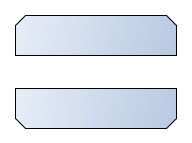
\includegraphics[scale=0.5]{pictures/lf06prog-pic/lf06prog-pap-schleife.png}
\end{itemize}

{\bf Struktogramm}~\\

Ein Nassi-Shneiderman-Diagramm, auch Strukogramm genannt, ist ein Diagrammtyp zur Darstellung von Programmentwürfen im Rahmen der strukturierten Programmierung. Struktogramme sind durch die DIN 66261 genormt.

Das Vorgehen zur Erstellung von Struktogrammen entspricht der Top-Down-Programmierung. Dabei wird zunächst ein Gesamtkonzept entwickelt und diese dann in Teilprobleme zerlegt bis nur noch elementare Grundstrukturen wie Sequenzen und Kontrollstrukturen übrig bleiben. Diese können dann als Strukogramm oder Programmablaufplan visualisiert werden.

\begin{itemize}
	\item Sequenz: Jede Anweisung wird in einen rechteckigen Strukturblock geschrieben. Die Strukturblöcke werden sequentiell durchlaufen.\\
	\item Einfache Verzweigung (Auswahl): Nur wenn die Bedingung zutreffend (wahr) ist, wird der Anweisungsblock 1 durchlaufen.\\
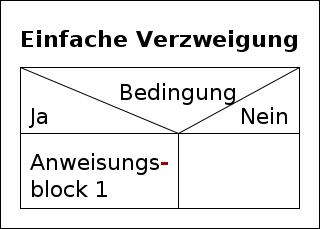
\includegraphics[scale=0.5]{pictures/lf06prog-pic/lf06prog-einfache-auswahl-struct.png}
	\item Zweifache Auswahl: Wenn die Bedingung zutreffend (wahr) ist, wird der Anweisungsblock 1 durchlaufen. Trifft die Bedingung nicht zu (falsch), wird der Anweisungsblock 2 durchlaufen. Ein Anweisungsblock kann aus einer oder mehreren Anweisungen bestehen. Austritt unten nach Abarbeitung des jeweiligen Anweisungsblocks.\\
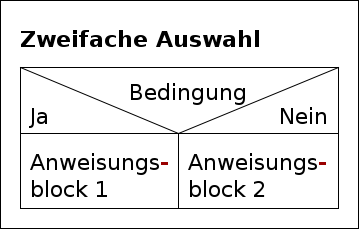
\includegraphics[scale=0.5]{pictures/lf06prog-pic/lf06prog-zweifache-auswahl-struct.png}
	\item Verschachtelte Auswahl: Es folgt eine weitere Bedingung. Die Verschachtelung ist ebenso im Nein-Fall (noch) möglich.\\
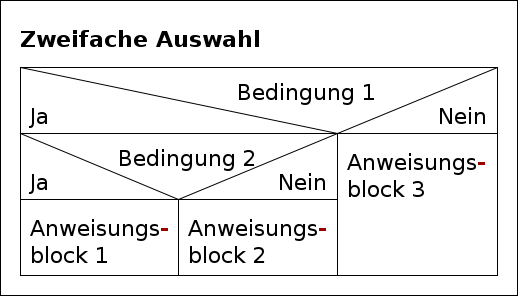
\includegraphics[scale=0.5]{pictures/lf06prog-pic/lf06prog-verschachtelte-auswahl-struct.png}
	\item Fallauswahl (Switch-Case): Besonders bei mehr als drei abzuprüfenden Bedingungen geeignet. Der Wert der Variable kann auf verschiedene Inhalte geprüft werden. Es wir dann der zugehörigen Anweisungsblock ausgeführt (switch, select). Eine Fallauswahl kann stets in eine verschachtelte Auswahl umgewandelt werden -- etwa wenn die später eingesetzte Programmiersprache Fallauswahl nicht beherrscht.\\
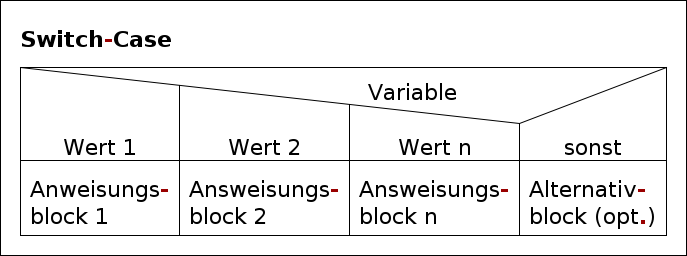
\includegraphics[scale=0.5]{pictures/lf06prog-pic/lf06prog-switch-case-struct.png}
\end{itemize}


%%% Ende: Struktogramm
%%%%%%%%%%%%%%%%%%%%%%%%%%%%%%%%%%%%%%%%%%%%%%%%%%%%%%%%%%%%%%%%%%%%%%%%%%%%%%%%

%%% Anfang: Verzweigung
\subsection{Verzweigungen und Schleifen}

In den folgenden Abschnitten werden wir uns mit IF-Verzweigungen sowie FOR- und WHILE-Schleifen in PHP beschäftigen. 

%%% Anfang: Verzweigung > Operatoren
\subsubsection{Vergleichsoperatoren, Verknüpfungen und Überprüfung von Eingabewerten}

PHP unterstützt ein Reihe von Vergleichsoperatoren. $=$ ist kein Vergleichsoperator, sondern eine Zuweisung.

\begin{tabular}{lll}
{\bf Operator} & {\bf Bedeutung} & {\bf Beispiel}\\
$==$ & Vergleich auf Gleichheit & \$zahl $== 5$\\
$===$ & Vergleich auf Typengleichheit & \$zahl $=== 5$\\
$!=$ & ungleich & \$zahl $!= 5$\\
$<$ & kleiner & \$zahl $< 5$\\
$<=$ & kleiner oder gleich & \$zahl $<= 5$\\
$>$ & größer & \$zahl $> 5$\\
$>=$ & größer oder gleich & \$zahl $>= 5$\\

\&\& & logisches Und & \$zahl $<= 1$ \&\& \$zahl $> 4$\\
|| & logisches Oder & \$zahl $== 0$ || \$zahl $< 0$\\
$!$ & logische Negation & $!$(\$zahl $<= 1$ \&\& \$zahl $> 4$)\\

\texttt{is\_numeric( \$var )} & Variable Zahl-? &\\
\texttt{isset( \$var )} & Existiert Variable? &\\
\texttt{empty( \$var )} & Variable leer? &\\
\end{tabular}

%%% Anfang: Verzweigung > IF
\subsubsection{IF}

Durch die Verwendung von IF lässt sich zwischen zwei Möglichkeiten auswählen, derjenigen, die ausgeführt wird, wenn die Bedingung zutrifft und derjenigen, für den Fall, dass die Bedingung nicht zutrifft. Generell kann die Bedingung einer IF-Konstruktion \texttt{true} oder \texttt{false} zurückgegeben.

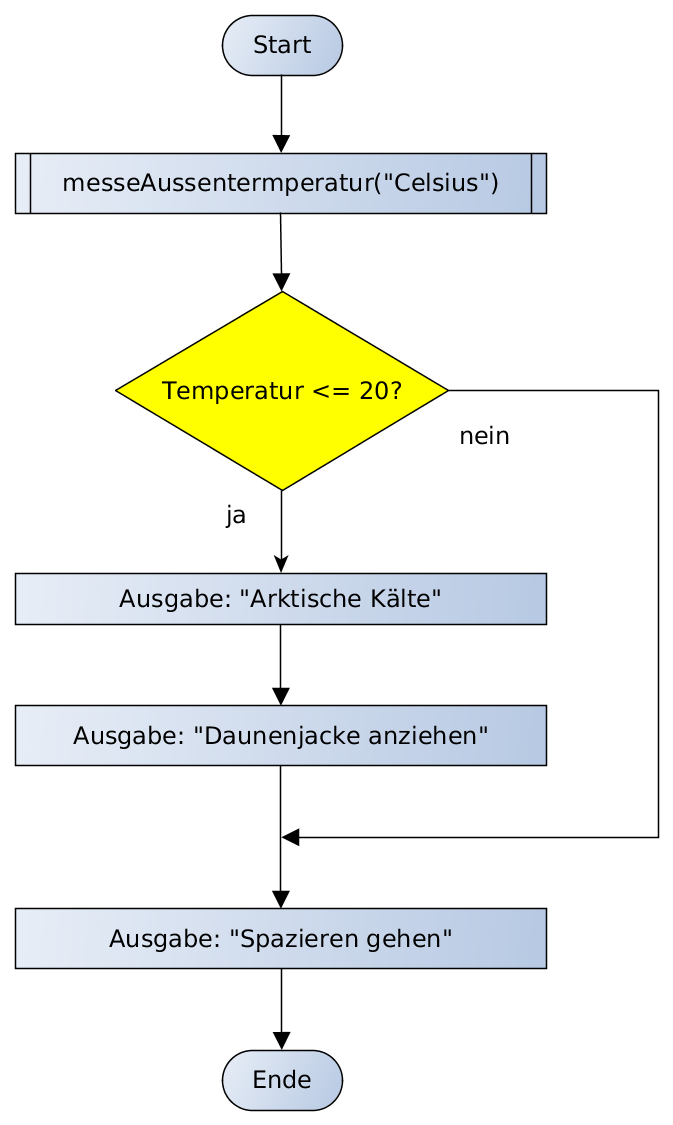
\includegraphics[scale=0.3]{pictures/lf06prog-pic/lf06prog-if-einseitig-pap.png}\\
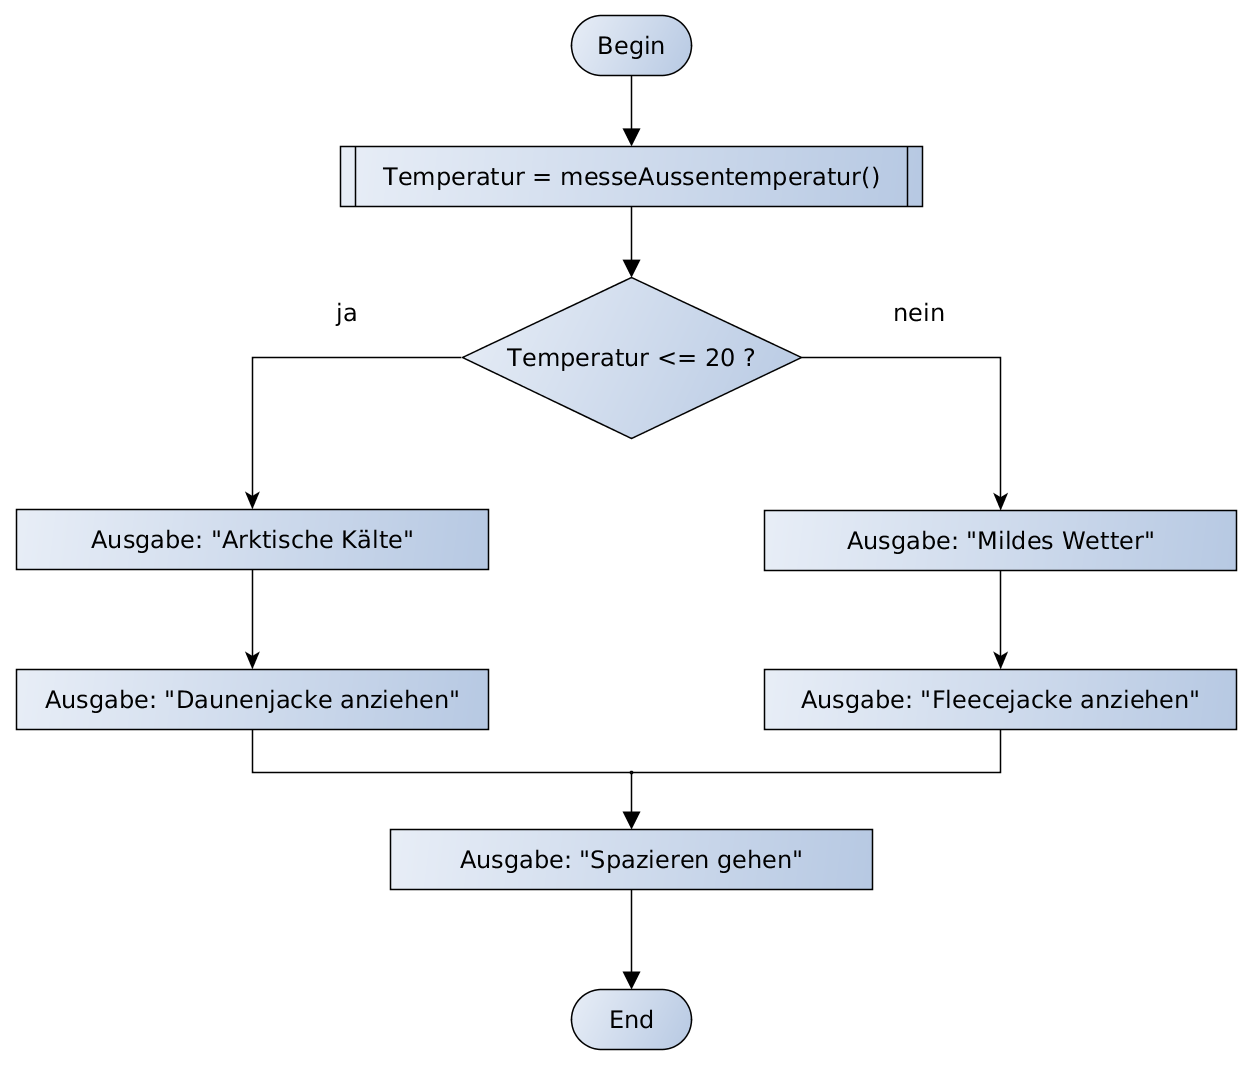
\includegraphics[scale=0.3]{pictures/lf06prog-pic/lf06prog-if-zweiseitig-pap.png}

%%% Anfang: Verzweigung > Switch
\subsubsection{Switch-Case}

Mit dem Konstrukt Switch-Case lässt sich eine Mehrfachauswahl (mehrseitige Auswahl) realisieren. Damit ist es im Gegensatz zu IF-Konstrukten möglich, zwischen beliebigen Werten statt zwischen \texttt{true} und \texttt{false} zu unterscheiden.

Die Variable, deren Wert geprüft wird, wird {\it Selektor} genannt. Der {\it Selektor} muss dafür vom Dateityp int oder char sein (in PHP auch string).

Im folgenden Listing ist eine Beispiel für Switch-Case-Konstrukte unter PHP gezeigt. Der Wert hinter \texttt{case} ist jeweils der Wert der Variable. Alle anderen Werte der Variable werden mit \texttt{default} abgefragt. Für das Beispiel bedeutet das, dass für alle Werte, die nicht $1$ oder $2$ sind, \ql ERR: not acceptable!\qr\ ausgegeben wird.

\lstinputlisting
	[basicstyle=\small,showstringspaces=false,caption={Ein Beispiel für Switch-Case-Anweisungen}
	\label{lst:Switch-Case},captionpos=b,language=PHP]
	{code/lf06prog-code/lf06prog-switch.case.php}
	
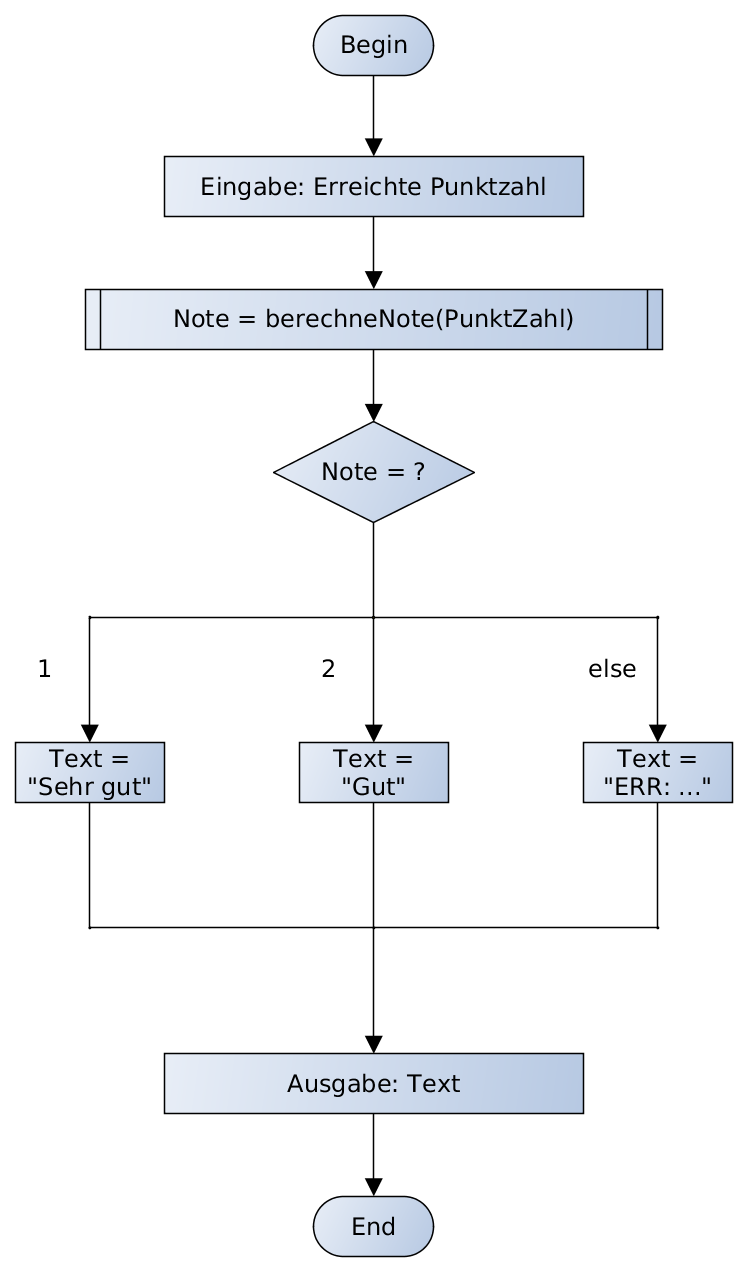
\includegraphics[scale=0.5]{pictures/lf06prog-pic/lf06prog-switch-case-pap.png}

%%% Anfang: Verzweigung > Schleifen
\subsubsection{Schleifen}

In Programmiersprachen stellt eine Schleife ein Kontrollstruktur dar. Sie wiederholt einen Anweisungsblock, den sogenannten Schleifenkörper, solange, wie eine Bedingung gültig ist oder bis eine Abbruchbedingung eintritt. Es werden vorprüfende und nachprüfende Schleifen unterschieden. Zu den vorprüfenden Schleifen gehören die kopfgesteuerte WHILE-Schleife, die FOR-Schleife und die Mengenschleife (FOREACH). Die fußgesteuerte WHILE-Schleife fällt zusammen mit der REPEAT-Schleife unter die nachprüfenden Schleifen.

\paragraph{FOR - Zählschleife}~\\

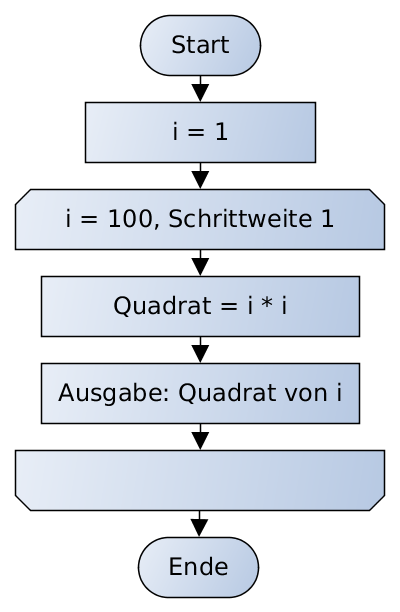
\includegraphics[scale=0.4]{pictures/lf06prog-pic/lf06prog-for-pap.png}
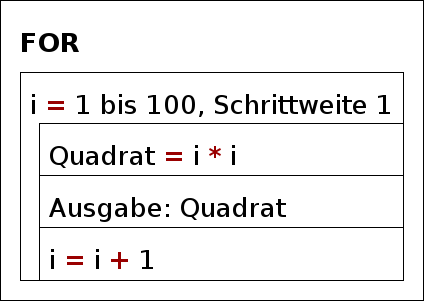
\includegraphics[scale=0.4]{pictures/lf06prog-pic/lf06prog-for-struct.png}

\lstinputlisting
	[basicstyle=\small,caption={Zählschleife, FOR}
	\label{lst:while-fuss},captionpos=b,language=PHP]
	{code/lf06prog-code/lf06prog-for.php}

\paragraph{WHILE}~\\

Die kopfgesteuerten WHILE-Schleifen unterscheiden sich von den fußgesteuerten dadruch, dass die Bedingung der Schleife bei letzterer erst nach dem einmaligen Durchlaufen der Schleife geprüft wird. Das bedeutet, dass fußgesteuerte Schleifen wie REPEAT immer mindestens einmal ausgeführt werden. Überspitzt lässt sich sagen, dass REPEAT erst schießt und dann fragt.

% While: Fuss
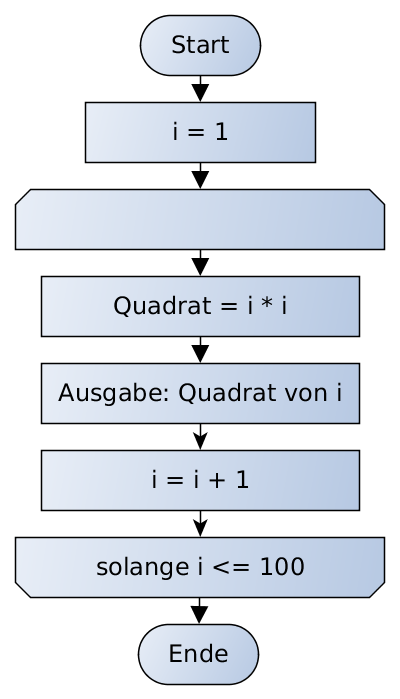
\includegraphics[scale=0.4]{pictures/lf06prog-pic/lf06prog-while-fuss-pap.png}
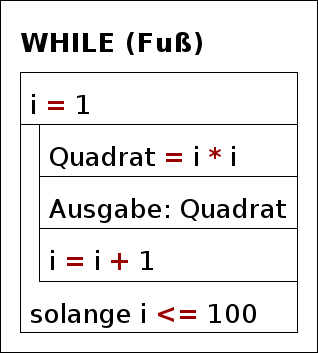
\includegraphics[scale=0.4]{pictures/lf06prog-pic/lf06prog-while-fuss-struct.png}

\lstinputlisting
	[basicstyle=\small,caption={Fussgesteuerte WHILE-Schleife}
	\label{lst:while-fuss},captionpos=b,language=PHP]
	{code/lf06prog-code/lf06prog-while-fuss.php}

% While: Kopf
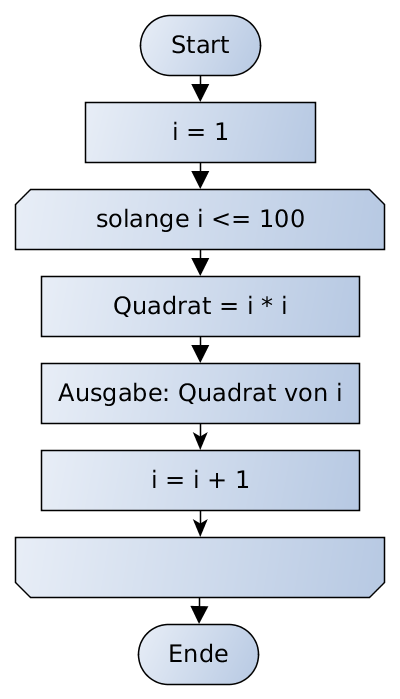
\includegraphics[scale=0.4]{pictures/lf06prog-pic/lf06prog-while-kopf-pap.png}
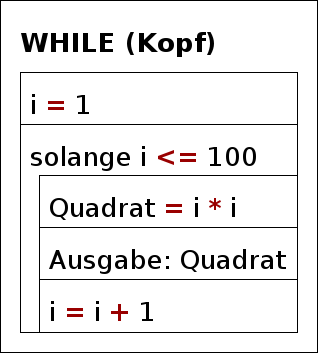
\includegraphics[scale=0.4]{pictures/lf06prog-pic/lf06prog-while-kopf-struct.png}

\lstinputlisting
	[basicstyle=\small,showstringspaces=false,caption={Kopfgesteuerte WHILE-Schleife}
	\label{lst:while-kopf},captionpos=b,language=PHP]
	{code/lf06prog-code/lf06prog-while-kopf.php}

%%% Anfang: Verzweigung > Arrays
\subsubsection{Arrays}

Der Datentyp Array kann beliebig viele, gleichartige Werte speichern. Im Gegensatz dazu können Variablen nur je einen Wert speichern. 

%%% Anfang: Verzweigung > Arrays > Index
\paragraph{Indexadressierte Arrays}~\\

Indexadressierte Arrays arbeiten mit Indizes, um auf die gespeicherten Werte zu verweisen. Im Listing [Nr] ist die Zuordnung und Ausgabe von indexadressierten Arrays am Beispiel von PHP gezeigt. Darin zeigt sich der Charakter eines Indizes: um einen Wert auszugeben, muss der entsprechende Index referenziert werden. Bevor eine Variable als Array verwendet werden kann, muss sie als solches definiert werden. Dies geschieht mit der Funktion \texttt{array()}. Eine Eigenheit von PHP besteht darin, dass es automatisch erkennt, dass eine Variable als Array benutzt werden soll. D.h., der Code aus dem Listing wäre auch ohne die Definition der Variablen als Arrays fehlerfrei. Im Listing zeigt sich auch die Eigenschaft von PHP, Arrays ohne explizite Indizes einen Index beginnend bei $0$ zu zuordnen. In anderen Programmiersprachen muss der Index immer explizit angegeben werden.

\lstinputlisting
	[basicstyle=\small,showstringspaces=false,caption={Indexadressierte Arrays in PHP}
	\label{lst:array-index},captionpos=b,language=PHP]
	{code/lf06prog-code/lf06prog-array-index.php}

%%% Anfang: Verzweigung > Arrays > Assozativ
\paragraph{Assoziative Arrays}~\\

%%% Ende: Verzweigung
%%%%%%%%%%%%%%%%%%%%%%%%%%%%%%%%%%%%%%%%%%%%%%%%%%%%%%%%%%%%%%%%%%%%%%%%%%%%%%%%

%%% Anfang: Aufgaben
\subsection{Aufgaben und Beispiele}

%%% Anfang: Aufgaben > LS01
\subsubsection{LS01: }

%%% Anfang: Aufgaben > LS02
\subsubsection{LS02: }

%%% Anfang: Aufgaben > LS03
\subsubsection{LS03: }

%%% Ende: Aufgaben
%%%%%%%%%%%%%%%%%%%%%%%%%%%%%%%%%%%%%%%%%%%%%%%%%%%%%%%%%%%%%%%%%%%%%%%%%%%%%%%%